\documentclass[twoside]{book}

% Packages required by doxygen
\usepackage{fixltx2e}
\usepackage{calc}
\usepackage{doxygen}
\usepackage[export]{adjustbox} % also loads graphicx
\usepackage{graphicx}
\usepackage[utf8]{inputenc}
\usepackage{makeidx}
\usepackage{multicol}
\usepackage{multirow}
\PassOptionsToPackage{warn}{textcomp}
\usepackage{textcomp}
\usepackage[nointegrals]{wasysym}
\usepackage[table]{xcolor}

% Font selection
\usepackage[T1]{fontenc}
\usepackage[scaled=.90]{helvet}
\usepackage{courier}
\usepackage{amssymb}
\usepackage{sectsty}
\renewcommand{\familydefault}{\sfdefault}
\allsectionsfont{%
  \fontseries{bc}\selectfont%
  \color{darkgray}%
}
\renewcommand{\DoxyLabelFont}{%
  \fontseries{bc}\selectfont%
  \color{darkgray}%
}
\newcommand{\+}{\discretionary{\mbox{\scriptsize$\hookleftarrow$}}{}{}}

% Page & text layout
\usepackage{geometry}
\geometry{%
  a4paper,%
  top=2.5cm,%
  bottom=2.5cm,%
  left=2.5cm,%
  right=2.5cm%
}
\tolerance=750
\hfuzz=15pt
\hbadness=750
\setlength{\emergencystretch}{15pt}
\setlength{\parindent}{0cm}
\setlength{\parskip}{3ex plus 2ex minus 2ex}
\makeatletter
\renewcommand{\paragraph}{%
  \@startsection{paragraph}{4}{0ex}{-1.0ex}{1.0ex}{%
    \normalfont\normalsize\bfseries\SS@parafont%
  }%
}
\renewcommand{\subparagraph}{%
  \@startsection{subparagraph}{5}{0ex}{-1.0ex}{1.0ex}{%
    \normalfont\normalsize\bfseries\SS@subparafont%
  }%
}
\makeatother

% Headers & footers
\usepackage{fancyhdr}
\pagestyle{fancyplain}
\fancyhead[LE]{\fancyplain{}{\bfseries\thepage}}
\fancyhead[CE]{\fancyplain{}{}}
\fancyhead[RE]{\fancyplain{}{\bfseries\leftmark}}
\fancyhead[LO]{\fancyplain{}{\bfseries\rightmark}}
\fancyhead[CO]{\fancyplain{}{}}
\fancyhead[RO]{\fancyplain{}{\bfseries\thepage}}
\fancyfoot[LE]{\fancyplain{}{}}
\fancyfoot[CE]{\fancyplain{}{}}
\fancyfoot[RE]{\fancyplain{}{\bfseries\scriptsize Generated by Doxygen }}
\fancyfoot[LO]{\fancyplain{}{\bfseries\scriptsize Generated by Doxygen }}
\fancyfoot[CO]{\fancyplain{}{}}
\fancyfoot[RO]{\fancyplain{}{}}
\renewcommand{\footrulewidth}{0.4pt}
\renewcommand{\chaptermark}[1]{%
  \markboth{#1}{}%
}
\renewcommand{\sectionmark}[1]{%
  \markright{\thesection\ #1}%
}

% Indices & bibliography
\usepackage{natbib}
\usepackage[titles]{tocloft}
\setcounter{tocdepth}{3}
\setcounter{secnumdepth}{5}
\makeindex

% Hyperlinks (required, but should be loaded last)
\usepackage{ifpdf}
\ifpdf
  \usepackage[pdftex,pagebackref=true]{hyperref}
\else
  \usepackage[ps2pdf,pagebackref=true]{hyperref}
\fi
\hypersetup{%
  colorlinks=true,%
  linkcolor=blue,%
  citecolor=blue,%
  unicode%
}

% Custom commands
\newcommand{\clearemptydoublepage}{%
  \newpage{\pagestyle{empty}\cleardoublepage}%
}

\usepackage{caption}
\captionsetup{labelsep=space,justification=centering,font={bf},singlelinecheck=off,skip=4pt,position=top}

%===== C O N T E N T S =====

\begin{document}

% Titlepage & ToC
\hypersetup{pageanchor=false,
             bookmarksnumbered=true,
             pdfencoding=unicode
            }
\pagenumbering{alph}
\begin{titlepage}
\vspace*{7cm}
\begin{center}%
{\Large Reverse Stairs }\\
\vspace*{1cm}
{\large Generated by Doxygen 1.8.13}\\
\end{center}
\end{titlepage}
\clearemptydoublepage
\pagenumbering{roman}
\tableofcontents
\clearemptydoublepage
\pagenumbering{arabic}
\hypersetup{pageanchor=true}

%--- Begin generated contents ---
\chapter{File Index}
\section{File List}
Here is a list of all documented files with brief descriptions\+:\begin{DoxyCompactList}
\item\contentsline{section}{/home/marques/\+Desktop/\+Cesium/\+D\+P\+U\+M/2\+\_\+reverse\+\_\+staircase/code\+\_\+golf/\+Marquinhos87/\+C/src/\hyperlink{stair_8h}{stair.\+h} }{\pageref{stair_8h}}{}
\end{DoxyCompactList}

\chapter{File Documentation}
\hypertarget{stair_8h}{}\section{/home/marques/\+Desktop/\+Cesium/\+D\+P\+U\+M/2\+\_\+reverse\+\_\+staircase/code\+\_\+golf/\+Marquinhos87/\+C/src/stair.h File Reference}
\label{stair_8h}\index{/home/marques/\+Desktop/\+Cesium/\+D\+P\+U\+M/2\+\_\+reverse\+\_\+staircase/code\+\_\+golf/\+Marquinhos87/\+C/src/stair.\+h@{/home/marques/\+Desktop/\+Cesium/\+D\+P\+U\+M/2\+\_\+reverse\+\_\+staircase/code\+\_\+golf/\+Marquinhos87/\+C/src/stair.\+h}}
{\ttfamily \#include $<$stdlib.\+h$>$}\newline
{\ttfamily \#include $<$stdio.\+h$>$}\newline
{\ttfamily \#include $<$string.\+h$>$}\newline
{\ttfamily \#include $<$ctype.\+h$>$}\newline
Include dependency graph for stair.\+h\+:
\nopagebreak
\begin{figure}[H]
\begin{center}
\leavevmode
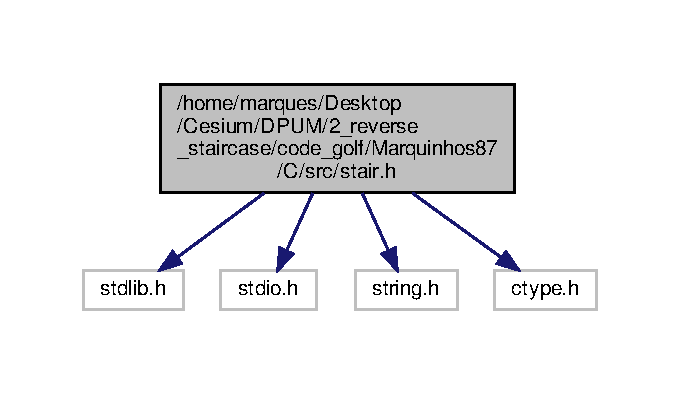
\includegraphics[width=327pt]{stair_8h__incl}
\end{center}
\end{figure}
\subsection*{Functions}
\begin{DoxyCompactItemize}
\item 
int \hyperlink{stair_8h_aba3d6e553970359c70d339243637b7b1}{verify} (char $\ast$l)
\item 
void \hyperlink{stair_8h_ae45efee5fa768da2b9735ea208c1b47d}{prt} (int tam)
\item 
int \hyperlink{stair_8h_a5d9faf356233ddf2e45046a4f502439b}{stair} (char $\ast$l)
\end{DoxyCompactItemize}


\subsection{Function Documentation}
\mbox{\Hypertarget{stair_8h_ae45efee5fa768da2b9735ea208c1b47d}\label{stair_8h_ae45efee5fa768da2b9735ea208c1b47d}} 
\index{stair.\+h@{stair.\+h}!prt@{prt}}
\index{prt@{prt}!stair.\+h@{stair.\+h}}
\subsubsection{\texorpdfstring{prt()}{prt()}}
{\footnotesize\ttfamily void prt (\begin{DoxyParamCaption}\item[{int}]{tam }\end{DoxyParamCaption})}

Function to print to stdout the result stair\+Case.


\begin{DoxyParams}{Parameters}
{\em tam} & Number of stairs to draw. \\
\hline
\end{DoxyParams}
\mbox{\Hypertarget{stair_8h_a5d9faf356233ddf2e45046a4f502439b}\label{stair_8h_a5d9faf356233ddf2e45046a4f502439b}} 
\index{stair.\+h@{stair.\+h}!stair@{stair}}
\index{stair@{stair}!stair.\+h@{stair.\+h}}
\subsubsection{\texorpdfstring{stair()}{stair()}}
{\footnotesize\ttfamily int stair (\begin{DoxyParamCaption}\item[{char $\ast$}]{l }\end{DoxyParamCaption})}

Function that calls the others to generate de final result.


\begin{DoxyParams}{Parameters}
{\em l} & String with the number of stairs. \\
\hline
\end{DoxyParams}
\begin{DoxyReturn}{Returns}
Return 0 if alright OK or 1 if something wrong 
\end{DoxyReturn}
\mbox{\Hypertarget{stair_8h_aba3d6e553970359c70d339243637b7b1}\label{stair_8h_aba3d6e553970359c70d339243637b7b1}} 
\index{stair.\+h@{stair.\+h}!verify@{verify}}
\index{verify@{verify}!stair.\+h@{stair.\+h}}
\subsubsection{\texorpdfstring{verify()}{verify()}}
{\footnotesize\ttfamily int verify (\begin{DoxyParamCaption}\item[{char $\ast$}]{l }\end{DoxyParamCaption})}

Function to verify if all characters pass to program are numbers


\begin{DoxyParams}{Parameters}
{\em l} & String pass to the program. \\
\hline
\end{DoxyParams}
\begin{DoxyReturn}{Returns}
Return 0 if alright OK or 1 if some character isn\textquotesingle{}t a number 
\end{DoxyReturn}

%--- End generated contents ---

% Index
\backmatter
\newpage
\phantomsection
\clearemptydoublepage
\addcontentsline{toc}{chapter}{Index}
\printindex

\end{document}
